% !TeX root = Presentation.tex
%

%-------System-----------------------------------------------------------------

\begin{frame}{Cart Pendulum}{The System}
  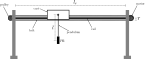
\includegraphics[width=1\textwidth]{figures/systemSetup}
\end{frame}

%-------Task--------------------------------------------------------------------

\begin{frame}{Cart Pendulum}{Swing-Up and Catch}
  \only<1|handout:0>
  {
  \vspace{-.3cm}
  \includegraphics[width=1\textwidth]{figures/cartPendulumAni/ani-0}
  }
  \only<2|handout:0>
  {
    \vspace{-.3cm}
    \animategraphics
    [ loop,
      autoplay,         %fps
      width=\linewidth ]{20}{figures/cartPendulumAni/ani-}{0}{119}
  }
  \only<0|handout:1>
  {
    \vspace{-.3cm}
    \includegraphics[width=1\textwidth]{figures/cartPendulumAni/ani-119}
  }
\end{frame}

%-------Results-----------------------------------------------------------------

\begin{frame}{Cart Pendulum}{Results}
  \begin{columns}[c]
    \column{.5\textwidth}
      \includegraphics[width=1\textwidth]{figures/Edelta_swing_p08}
    \column{.5\textwidth}
      \includegraphics[width=1\textwidth]{figures/phase_swing_p08}
  \end{columns}
  \vspace{12pt}
  \begin{columns}[c]
    \column{.5\textwidth}
      \begin{itemize}
        \item Energy based control
      \end{itemize}
    \column{.5\textwidth}
      \begin{itemize}
        \item Heteroclinic orbit
      \end{itemize}
  \end{columns}
\end{frame}

\begin{frame}{Cart Pendulum}{Results}
  \begin{columns}[c]
    \column{.5\textwidth}
      \includegraphics[width=.99\textwidth]{figures/theta_swingNslide}
    \column{.5\textwidth}
      \includegraphics[width=1.031\textwidth]{figures/x_swingNslide}
      \vspace{-10pt}
  \end{columns}
  \begin{columns}[c]
    \column{.5\textwidth}
    \begin{itemize}
      \item Swing-up
      \item Catch using sliding mode
    \end{itemize}
    \column{.5\textwidth}
    \begin{itemize}\centering
      \item Cart maintained near zero
    \end{itemize}
  \end{columns}
\end{frame}

%-------Twin System-------------------------------------------------------------

\begin{frame}{Twin Pendulum}{The System}
  \vspace{-.5cm}\hspace{1cm}
  \includegraphics[width=.8\textwidth]{figures/twinSetupLabled}
\end{frame}

%-------Task--------------------------------------------------------------------

\begin{frame}{Twin Pendulum}{Swing-Up and Catch}
  \only<1|handout:0>
  {
    \vspace{-.3cm}
    \includegraphics[width=1\textwidth]{figures/twinPendulumAni/ani-0}
  }
  \only<2|handout:0>
  {
    \vspace{-.3cm}
    \animategraphics
    [ loop,
      autoplay,         %fps
      width=\linewidth ]{12}{figures/twinPendulumAni/ani-}{0}{148}
  }
  \only<0|handout:1>
  {
    \vspace{-.3cm}
    \includegraphics[width=1\textwidth]{figures/twinPendulumAni/ani-148}
  }
\end{frame}

%-------Results-----------------------------------------------------------------

\begin{frame}{Twin Pendulum}{Results}
  \begin{columns}[c]
    \column{.5\textwidth}
      \includegraphics[width=1\textwidth]{figures/thetaCatch}
    \column{.5\textwidth}
      \includegraphics[width=1\textwidth]{figures/xCatch}
  \end{columns}
  \begin{columns}[c]
    \column{.5\textwidth}
    \begin{itemize}\vspace{12pt}
      \item LQR stabilizing both pendulums
    \end{itemize}
    \column{.5\textwidth}
    \begin{itemize}\centering
      \item Cart maintained near zero
    \end{itemize}
  \end{columns}
\end{frame}

\begin{frame}{Twin Pendulum}{Results}
  \begin{columns}[c]
    \column{.5\textwidth}
      \includegraphics[width=.85\textwidth]{figures/thetaSwingAttempt}
    \column{.5\textwidth}
      \includegraphics[width=.85\textwidth]{figures/phaseSwingAttempt}
  \end{columns}
  \begin{columns}[c]
    \column{.5\textwidth}
    \begin{itemize}\vspace{-12pt}
      \item Swing-up not reaching equilibrium
    \end{itemize}
    \column{.5\textwidth}
    \begin{itemize}
      \item Pendulum 1 overshoots before pendulum 2 reaches equilibrium
    \end{itemize}
  \end{columns}
\end{frame}

%-------New Results-------------------------------------------------------------

\begin{frame}{Twin Pendulum}{New Results}
  \begin{columns}[c]
    \column{.5\textwidth}
      \includegraphics[width=1\textwidth]{figures/thetaCatch}
    \column{.5\textwidth}
      \includegraphics[width=1\textwidth]{figures/xCatch}
  \end{columns}
  \begin{columns}[c]
    \column{.5\textwidth}
    \begin{itemize}\vspace{12pt}
      \item Sliding mode stabilizing both pendulums
    \end{itemize}
    \column{.5\textwidth}
    \begin{itemize}\centering
      \item Cart maintained near zero
    \end{itemize}
  \end{columns}
\end{frame}

\begin{frame}{Twin Pendulum}{New Results}
  \centering
  \includegraphics[width=.6\textwidth]{figures/thetaSlidingModeCatchAttempt}
  \begin{itemize}\vspace{6pt}
    \item Sliding mode attempt at catching both pendulums after swing-up
  \end{itemize}
\end{frame}

\begin{frame}{Twin Pendulum}{New Results}
  \begin{columns}[c]\vspace{-12pt}
    \column{.5\textwidth}
      \includegraphics[width=.95\textwidth]{figures/EdeltaSlidingModeCatchAttempt}
    \column{.5\textwidth}
      \includegraphics[width=.95\textwidth]{figures/phaseSlidingModeCatchAttempt}
  \end{columns}
  \begin{columns}[c]
    \column{.5\textwidth}
    \begin{itemize}
      \item Energy references reached
    \end{itemize}
    \column{.5\textwidth}
    \begin{itemize}\centering
      \item Equilibrium reached
    \end{itemize}
  \end{columns}
\end{frame}